\documentclass[10pt, a4paper, italian]{article}
\usepackage[T1]{fontenc}
\usepackage[utf8]{inputenc}
\usepackage{amsmath, amssymb, amsthm, thmtools, amsfonts, mathtools}
\usepackage{nicefrac}
\usepackage{calc}
\usepackage[pdftex, hyperindex, plainpages=false]{hyperref}
\usepackage[nameinlink]{cleveref} %load before classicthesis (clash)
%\usepackage[nochapters,pdfspacing]{classicthesis}
\usepackage{siunitx}
\usepackage[siunitx]{circuitikz}

\usepackage[a4paper]{geometry}
\usepackage{float}
\usepackage{mdframed}
\usepackage{titling}
\usepackage{booktabs}
\usepackage{graphicx}
\usepackage{caption, subcaption}
\usepackage{xcolor}
\usepackage[italian]{babel}
\usepackage{pgfplots}
\usepackage{listings}
%\usepackage{lmodern}
\usepackage{url}
\usepackage{enumitem}
\usepackage{tikz} %loads after classicthesis (xcolor incompat)

% lets graphicx know path where figures to be included are found
\graphicspath{{../figs/}}
\makeatletter
\def\input@path{{../figs/}}
%or: \def\input@path{{/path/to/folder/}{/path/to/other/folder/}}
\makeatother

% tikz pgf plots setup
\usepgfplotslibrary{external}
\pgfplotsset{compat=1.15}
%\tikzexternalize

% spaces and significant digits/figures for measurements
\sisetup{free-standing-units, space-before-unit, number-unit-product = \;,
scientific-notation = false, round-mode = figures, round-precision = 1,}

% turns all (hyperlinked) references black [default is blue]
\hypersetup{
	linktoc=all,
	colorlinks=true,
	linkcolor=black
}

% code listings config
%\lstset{
%language=Python,
%basicstyle=\ttfamily,
%columns=fullflexible,
%keepspaces=true,
%}

% mdframed (for boxed text) configuration
\mdfsetup{linewidth=0.6pt}

% Default fixed font does not support bold face
\DeclareFixedFont{\ttb}{T1}{txtt}{bx}{n}{12} % for bold
\DeclareFixedFont{\ttm}{T1}{txtt}{m}{n}{12}  % for normal

% Custom colors
\usepackage{color}
\definecolor{deepblue}{rgb}{0,0,0.5}
\definecolor{deepred}{rgb}{0.6,0,0}
\definecolor{deepgreen}{rgb}{0,0.5,0}

% Commands 
\newcommand{\executeiffilenewer}[3]{%
	\ifnum\pdfstrcmp{\pdffilemoddate{#1}}%
		{\pdffilemoddate{#2}}>0%
	{\immediate\write18{#3}}\fi%
}
% input .svg --> .pdf_tex graphs
%\newcommand{\includesvg}[1]{%
%	\executeiffilenewer{#1.svg}{#1.pdf}%
%	{inkscape -z -D --file=#1.svg %
%	--export-pdf=#1.pdf --export-latex}%
%	\input{#1.pdf_tex}%
%}
% Thanks UniPi's Department of Physics E. Fermi
\newcommand{\thanksdf}{(\thanks{Dipartimento di Fisica E.~Fermi,%
Universit\`a di Pisa - Pisa, Italy.}\;)}

% hyperlink to email address
\newcommand{\mail}[1]{\href{mailto:#1}{\textsf{#1}}}

% \vec for bold vectors, instead of overarrows (now "\arrvec")
\let\arrvec=\vec
\renewcommand{\vec}[1]{\boldsymbol #1}
% replaces straight phi with slanted phi
\renewcommand{\phi}{\varphi}
% replaces straight eps with curved epsilon
\newcommand{\eps}{\varepsilon}
% abbreviation for (sub_/super^)scripts of \lim, \sum,... in inline math
\newcommand{\ds}{\displaystyle}

% blackboard/number set letters
\newcommand{\CC}{\mathbb C}
\newcommand{\HH}{\mathbb H}
\newcommand{\KK}{\mathbb K}
\newcommand{\NN}{\mathbb N}
\newcommand{\PP}{\mathbb P}
\newcommand{\QQ}{\mathbb Q}
\newcommand{\RR}{\mathbb R}
\newcommand{\ZZ}{\mathbb Z}

\newcommand{\Abs}[1]{{\left\Vert #1\right\Vert}}
\newcommand{\enclose}[1]{{\left( #1 \right)}}
\newcommand{\Enclose}[1]{{\left[ #1 \right]}}
\newcommand{\floor}[1]{\left\lfloor #1 \right\rfloor}
\newcommand{\ceil}[1]{\left\lceil #1 \right\rceil}
\newcommand{\To}{\rightrightarrows}

% Math operators
\DeclareMathOperator{\divergence}{div}
\renewcommand{\div}{\divergence}
\DeclareMathOperator{\Imaginarypart}{Im}
\renewcommand{\Im}{\Imaginarypart}
\DeclareMathOperator{\Realpart}{Re}
\renewcommand{\Re}{\Realpart}
%\DeclareMathOperator{\arg}{arg}
\DeclareMathOperator{\tg}{tg}
\DeclareMathOperator{\arctg}{arctg}
\DeclareMathOperator{\settsinh}{settsinh}
\DeclareMathOperator{\settcosh}{settcosh}
\DeclareMathOperator{\tr}{tr}
\DeclareMathOperator{\im}{im}
\DeclareMathOperator{\sgn}{sgn}
\DeclareMathOperator{\diag}{diag}

\DeclarePairedDelimiter{\norm}{\lVert}{\rVert}
\DeclarePairedDelimiter{\scalar}{\langle}{\rangle}

% Logarithm with arbitrary base.
% -> log_10
\newcommand{\llog}[1][10]{\log_{#1}}

% Absolute value.
% -> |x|
\newcommand{\abs}[1]{\left| #1 \right|}

% Powers.
% -> x^a
\newcommand{\power}[2][2]{\left( #2 \right)^{#1}}

% Square.
% -> x^2
\newcommand{\sq}[1]{\power[2]{#1}}

% Expansion of the binomial coefficient.
% -> n1!/(n2!(n1 - n2)!)
\newcommand{\binomexpr}[2]{\frac{#1!}{#2!(#1 - #2)!}}

% Expression evaluation at a given point with square brackets.
% -> [x]_{a}
\newcommand{\at}[2]{\left[ #1\right]_{\makebox[-1pt][l]{${\scriptstyle#2}$}}}

% Expression evaluation in an interval.
% -> [x] _{a}^{b}
\newcommand{\eval}[3]{\left.#1%
  \right|_{\makebox[-1pt][l]{${\scriptstyle#2}$}}^{\makebox[-1pt][l]{${\scriptstyle#3}$}}}

% Upright d in math mode (for differentials).
% -> d
\newcommand{\ud}{\mathrm{d}}

% Differential.
% -> dx
\newcommand{\diff}[1][x]{\,\ud{#1}}

% Base command for defining derivatives.
% -> df/dx or d^kf/dx^k
\newcommand{\basederivative}[4][]{%
  \displaystyle%
  \ifx\\#1\\\frac{#4#2}{#4#3}%
  \else%
  \frac{#4^#1#2}{#4#3^#1}%
  \fi%
}

% Total derivative.
% -> df/dx(x) or d^kf/dx^k(x)
\newcommand{\td}[4][]{%
  \basederivative[#1]{#2}{#3}{\ud}%
  \ifx\\#4\\%
  \else%
  \mkern-4mu\left(#4\right)%
  \fi%
}

% Partial derivative.
% -> df/dx(x) or d^kf/dx^k(x)
\newcommand{\pd}[4][]{%
  \basederivative[#1]{#2}{#3}{\partial}%
  \ifx\\#4\\%
  \else%
  \mkern-4mu\left(#4\right)%
  \fi%
}

\newcommand{\intinf}{\int_{-\infty}^{\infty}\!\!\!}

\newcommand{\cinterval}[2]{\left[\, #1,~#2 \,\right]}

\newcommand{\linterval}[2]{\left[\, #1,~#2 \,\right)}

\newcommand{\rinterval}[2]{\left(\, #1,~#2 \,\right]}

\newcommand{\ointerval}[2]{\left(\, #1,~#2 \,\right)}

\newcommand{\prob}[1]{\displaystyle P\left(#1\right)}

\newcommand{\pvalue}{\emph{$p$-value}}

\newcommand{\cond}{\,|\,}

\newcommand{\expect}[1]{\displaystyle E\left[#1\right]}

\newcommand{\mom}[2][]{\displaystyle {\cal M}_{#2}\ifx\\#1\\\else(#1)\fi}

\newcommand{\momalg}[1]{\displaystyle \lambda_{#1}}

\newcommand{\momcen}[1]{\displaystyle \mu_{#1}}

\newcommand{\skewness}{\displaystyle \gamma_1}

\newcommand{\kurtosis}{\displaystyle \gamma_2}

\newcommand{\charf}[1][x]{\phi_{#1}}

\newcommand{\momgenf}[1][x]{M_{#1}}

\newcommand{\fwhm}{{\scriptstyle \textsc{FWHM}}}

\newcommand{\hwhm}{{\scriptstyle \textsc{HWHM}}}

\newcommand{\median}{\mu_{\nicefrac{1}{2}}}

\newcommand{\var}[1]{\ensuremath{\text{Var}\left(#1\right)}}

\newcommand{\cov}[2]{\ensuremath{\text{Cov}\left(#1, #2\right)}}

\newcommand{\corr}[2]{\ensuremath{\text{Corr}\left(#1, #2\right)}}

\newcommand{\like}{\mathcal L}

\newcommand{\likelihood}[2][]{\like\ifx\\#2\\\else(#2\ifx\\#1\\\else;#1\fi)\fi}

\newcommand{\chisq}{\ensuremath{\chi^2}}

\newcommand{\chisquare}[2][]{\chisq\ifx\\#2\\\else(#2\ifx\\#1\\\else;#1\fi)\fi}

\newcommand{\loglikelihood}[2][]{\log\likelihood[#1]{#2}}

\newcommand{\pdf}[3][]{#2(#3\ifx\\#1\\\else;#1\fi)}

\newcommand{\binomialpdf}[2][]{\pdf[#1]{\mathcal B}{#2}}

\newcommand{\multinomialpdf}[2][]{\pdf[#1]{\mathcal M}{#2}}

\newcommand{\poissonpdf}[2][]{\pdf[#1]{\mathcal P}{#2}}

\newcommand{\uniformpdf}[2][]{\pdf[#1]{u}{#2}}

\newcommand{\exponentialpdf}[2][]{\pdf[#1]{\varepsilon}{#2}}

\newcommand{\gausspdf}[2][]{\pdf[#1]{N}{#2}}

\newcommand{\chisquarepdf}[2][]{\pdf[#1]{\wp}{#2}}

\newcommand{\cauchypdf}[2][]{\pdf[#1]{c}{#2}}

\newcommand{\erf}[1]{\ensuremath{\text{erf}\left(#1\right)}}

\newcommand{\dccases}[4][]{#2 \ifx\\#2\\\else=\fi %
  \begin{cases}
    \displaystyle #3 & \text{per variabili discrete}\\
    \displaystyle #4 & \text{per variabili continue}#1
  \end{cases}
}
% sub/super-scriptable for all symbol as math operator 
\newcommand\Scaleforall[1]{\vcenter{\hbox{\scalefont{#1}$\forall$}}}

\DeclareMathOperator*\forevery{%
  \vphantom\sum
  \mathchoice{\Scaleforall{2}}{\Scaleforall{1.4}}{\Scaleforall{1}}{\Scaleforall{0.75}}}
\usepackage{multicol}
\usepackage{diagbox}
\geometry{left=2cm, right=2cm, top=2cm, bottom=2cm}

% indexes subsections with letters, sections with numbers (1.a, 1.b, ...)
\renewcommand{\thesubsection}{\thesection.\alph{subsection}}

% lets graphicx know path where figures to be included are found
\graphicspath{{../figs/}}

\author{Gruppo 1.AC \\ Matteo Rossi, Bernardo Tomelleri}
\title{EsD2: Costruzione di D-Latch, contatori e shift-register}
\begin{document}
\date{\today}
\maketitle

\section{Misura componenti dei circuiti}
Riportiamo per completezza il valore della tensione continua di
alimentazione per i circuiti integrati misurata con il multimetro
\[
V_{CC} = 4.99 \pm 0.03 \si{\V}
\]

e il valore di capacità del condensatore di disaccoppiamento che collega le
linee di alimentazione a massa (sempre misurato con il multimetro)
\[
C_d = 97 \pm 4 \; \si{n\F}
\]

%=======================
\section{D-Latch con Enable}\label{sec: dlatch}
\subsection{Costruzione del circuito}
Si è costruito un circuito D-Latch secondo lo schema mostrato in
\cref{schm: dlatch} utilizzando le porte NAND di due integrati SN74LS00.
\begin{figure}
\centering
\begin{circuitikz}
    \draw (0,2.4) node[american nand port,label=north:R] (mynand1){};
    \draw (0,0) node[american nand port,label=south:S] (mynand2){};
    \draw (2.5,2.4) node[american nand port] (mynand3){};
    \draw (2.5,0) node[american nand port] (mynand4){};
    \draw (-3.5,0.5) node[american nand port,label=left:$\bar{D}$ NOT,
    rotate = 270] (mynand5){};
    \draw (-2,1.2) node[circ, label=left:$E$](E){}; 

	\draw (mynand3.out) to[short] ++(0,-1) to[short] ++(-2,0) |- (mynand4.in 1);
	\draw (mynand4.out) -- ++(1,0) node[circ, label=right:$\overline{Q}$]{};
	\draw (mynand3.out) -- ++(1,0) node[circ, label=right:$Q$]{};
	\draw (mynand4.out) to[short] ++(0,1) to[short] ++(-1.8,0) |- (mynand3.in 2);
    \draw (mynand1.out) |- (mynand3.in 1);
    \draw (mynand2.out) |- (mynand4.in 2);
    \draw (mynand5.in 1) |- (mynand5.in 2);
    \draw (mynand5.in 2) |- (mynand1.in 1);
    \draw (mynand1.in 1) -- ++ (-3,0) node[circ, label=left:$D$]{};
    \draw (mynand5.out) |- (mynand2.in 2);
    \draw (mynand2.in 1) |- (E);
    \draw (mynand1.in 2) |- (E);
\end{circuitikz}
\caption{Schema logico del circuito $D$-Latch (con Enable) realizzato
\label{schm: dlatch}}
\end{figure}

Per studiarne il comportamento generiamo nei due pin DIO 0 (DATA) e DIO 1
(ENABLE) dell'AD2 due segnali di clock di frequenza $f = \SI{1}{k\hertz}$ e
sfasati tra loro di $\pm \SI{90}{\degree}$ agli ingressi $D$ ed $E$ del
circuito. 

\subsection{Analisi del funzionamento del circuito}
Il circuito è composto da un Latch $RS$ i cui ingressi sono collegati a due
porte NAND, di cui un ingresso per ciascuna è collegato all'input $E$, mentre
gli altri due ingressi sono collegati l'uno al segnale opposto dell'altro
tramite una porta NOT (in figura la porta NAND più in alto tra le due $(R)$ è
collegata all'input $D$, mentre quella più in basso $(S)$ a $\overline{D}$).

L'equazione fondamentale del circuito è quindi data dalla
\begin{equation}
Q(t + \Delta t) = \overline{\overline(D \cdot E)} +
\overline{(\overline{D} \cdot E)} \cdot Q(t) =
E \cdot D + \overline{E} \cdot Q(t)
\end{equation}
da cui si può ricavare la corrispondente tabella di verità
\begin{table}
\begin{center}
    \begin{tabular}{cccc}
      \toprule
      $E$ & $D$     & $Q(t)$  & $ Q(t + \Delta t)$ \\
      \midrule
      \midrule
      0     & X & 0         & 0 \\
      0     & X & 1         & 1 \\
      1     & 0         & X & 0 \\
      1     & 1         & X & 1 \\
      \bottomrule
    \end{tabular}
\end{center}
\caption{Tabella di verità del circuito $D$-Latch con Enable (con X si indica
valore logico indefinito/don't care) \label{tab: dlatch}}
\end{table}

Come si può vedere dalla tabella di verità (\cref{tab: dlatch}) l'uscita $Q$
funge da memoria a un bit se $E$ è al livello logico basso (stato di HOLD),
mentre assume il valore logico dell'input $D$ quando il segnale di ENABLE è
acceso.
Questo rende il valore dell'uscita indipendente dalle caratteristiche
temporali delle porte NAND e protegge il circuito dallo stato proibito di
oscillazione/racing $R = S = 1$ da cui è affetto il semplice $RS$-Latch.

\subsection{Verifica della tabella di verità del Latch}
Per conferma del corretto funzionamento del Latch possiamo confrontare
le uscite ottenute da un'acquisizione con Logic Analyzer con i valori
riportati in \cref{tab: dlatch} inviando all'ingresso del circuito con
Patterns due segnali di clock sfasati tra loro di $\phi = \SI{90}{\degree}$.
\begin{figure}[htbp]
    \centering
    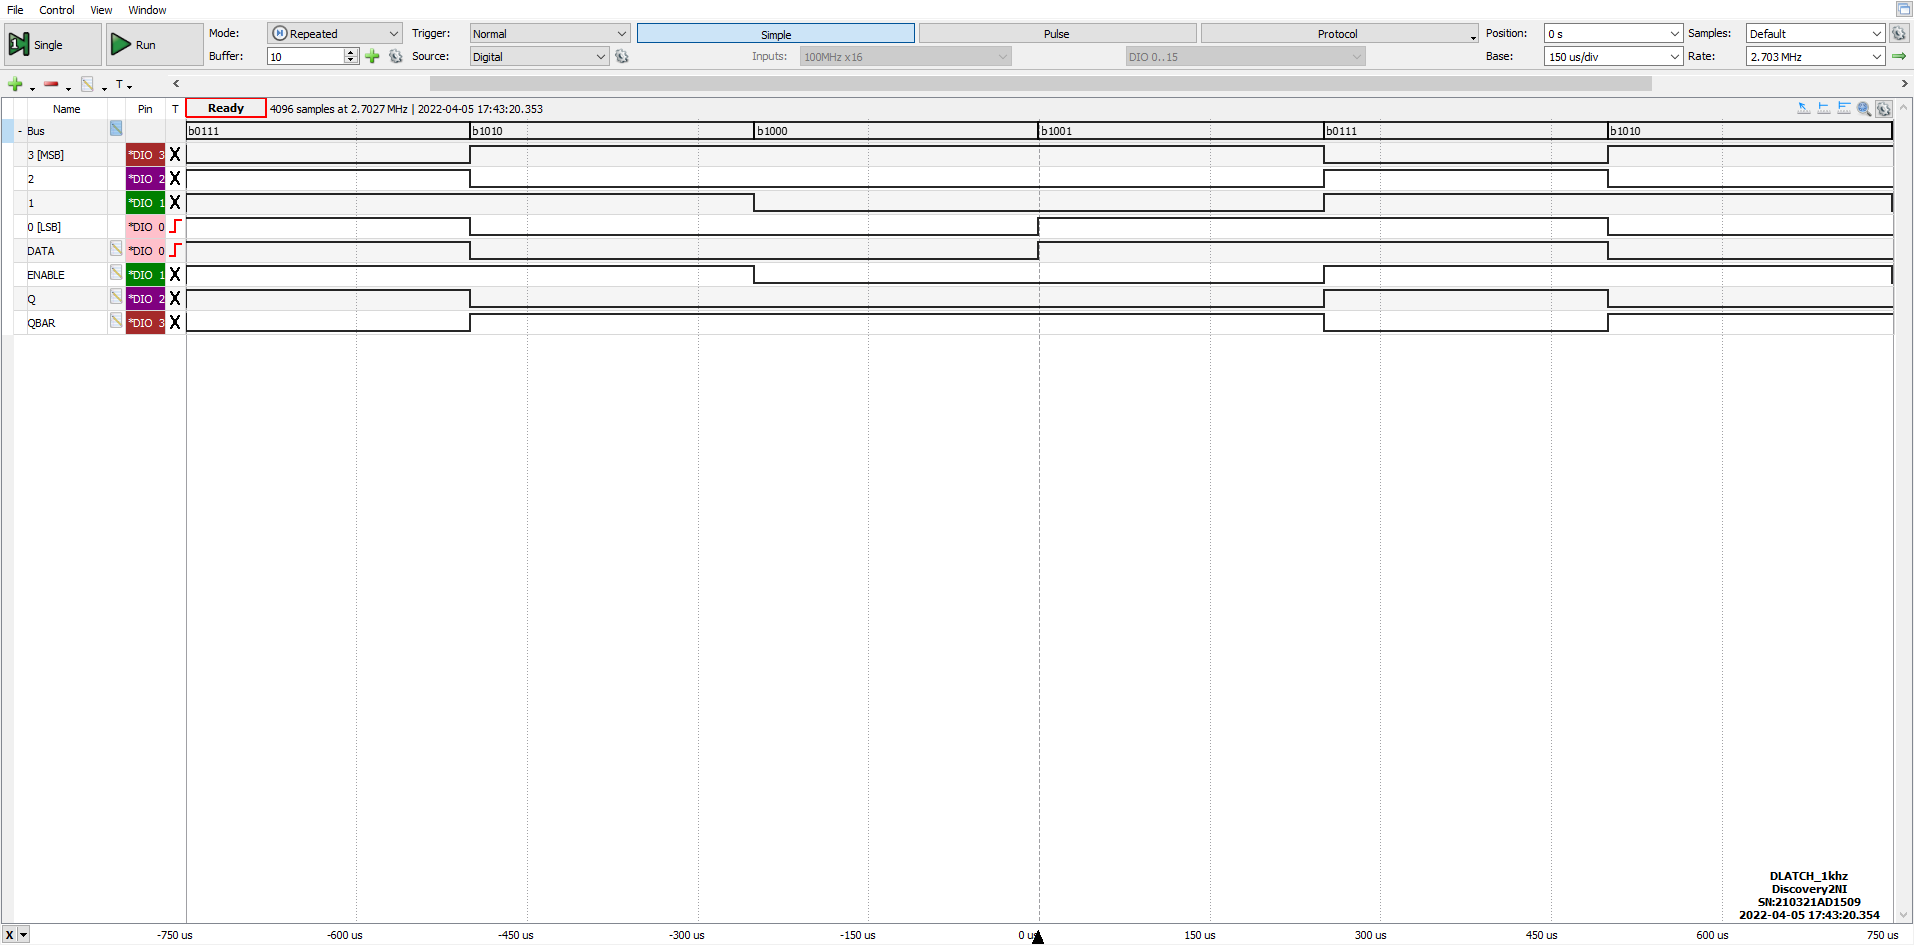
\includegraphics[width=\textwidth]{dlatch}
    \caption{Acquisizione di un ciclo completo (frequenza 1 kHz) con Logic
    Analyzer dei segnali in ingresso ($D =$ DIO 0, $E =$ DIO 1) e in uscita
    ($Q =$ DIO 2, $\overline{Q} =$ DIO 3) dal D-Latch.
    \label{fig: dlatch}}
\end{figure}
\begin{figure}[htbp]
	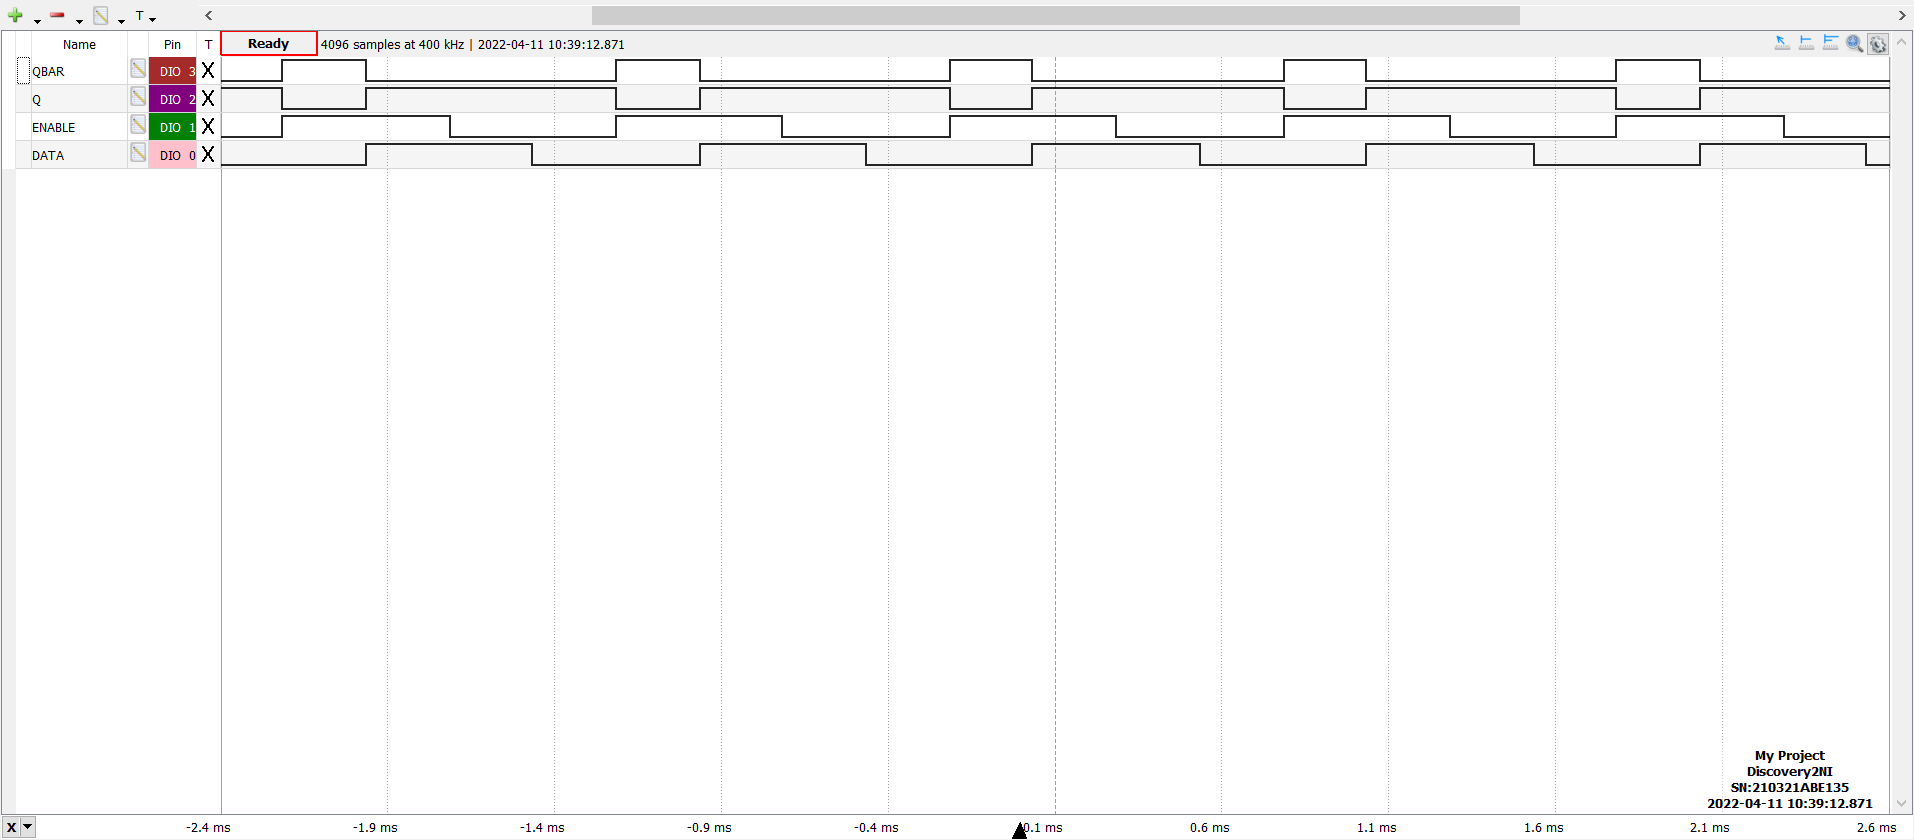
\includegraphics[width=\textwidth]{latch2}
	\caption{Acquisizione temporale con Logic dei segnali in ingresso uscita dal
	D-Latch per $\phi = -\SI{90}{\degree}$.
	\label{fig: Log_DLATCH2}}
\end{figure}

Dalle \cref{fig: dlatch} e \cref{fig: Log_DLATCH2} si osserva come durante lo
stato basso di Enable il segnale in uscita rimanga costante rispetto a
variazioni del segnale in $D$, mentre quando
$E = 1 \implies Q(t + \Delta t) = D$ coerentemente con quanto previsto dalla
tabella di verità.

\subsection{Misura dei tempi del ritardo nelle transizioni di stato}
Si riescono a distinguere due diverse transizioni dei segnali in ingresso per
ciascun valore di sfasamento tra i due segnali di clock in $D$ ed $E$;
per $\phi = \SI{90}{\degree}$:
\begin{enumerate}
\item $D: 1 \to 0$, $E \coloneqq 1$ \label{item: Dfall}
\item $D \coloneqq 1$, $E: 0 \to 1$. \label{item: Erise}

Mentre per $\phi = - \SI{90}{\degree} = 270 \; \si{\degree}$:
\item $D \coloneqq 0$, $E: 0 \to 1$ \label{item: Efall}
\item $D: 0 \to 1$, $E \coloneqq 1$. \label{item: Drise}
\end{enumerate}


Il ritardo di durata maggiore risulta quello della transizione
\ref{item: Dfall} dell'input $D$ da alto a basso ($40 \pm 10$ ns).

Dalle misure prese con i cursori dell'oscilloscopio (a cui associamo come
incertezza il contributo dato dalle specifiche del datasheet, tenendo conto
dell'instabilità delle tracce sullo schermo) troviamo
\begin{align*}
    t_{PLH}= 11 \pm 1 \; \si{n\s} \\
    t_{PHL}= 35 \pm 2 \; \si{n\s}
\end{align*}

Dalle specifiche del DS si trova che i tempi di propagazione tipici e massimi
per una singola porta NAND sono:
\begin{table}[htbp]
\centering
\begin{tabular}{cccc}
	& typ & max & [units] \\
    $t\ped{PLH}$ & $11$ & $22$ & \si{n\s} \\
    $t\ped{PHL}$ & $7$ & $15$ & \si{n\s}
\end{tabular}
\end{table}

%=======================
\section{Shift-register con edge-triggered D-Flip Flop}
\subsection{Costruzione del circuito}
Si vuole ora costruire uno Shift Register a 4 bit a partire dagli integrati della serie SN74LS74, secondo lo schema in \cref{fig: schem_shift} e verificarne il funzionamento.
\begin{figure}[htbp]
\centering
	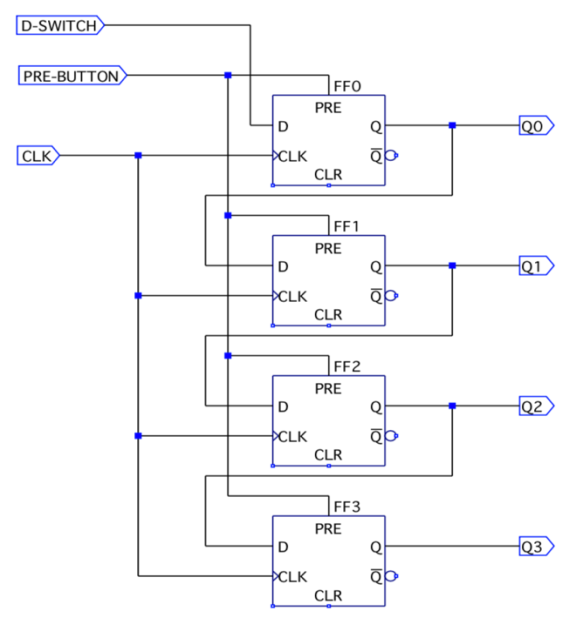
\includegraphics[width=0.6\textwidth]{schem_shift}
	\caption{\label{fig: schem_shift}}
\end{figure}

\subsection{Verifica della sincronia delle uscite tramite PRESET}
Per prima cosa dopo aver montato il circuito verifichiamo la sincronicità delle commutazioni delle uscite.
Dopo aver controllato che le uscite Q0, Q1, Q2 e Q4 fossero nello stato 0000, mantenendo il segnale di clock e il D-Switch scollegati abbiamo utilizzato la funzione StaticIO di wavegen per pilotare il pin PRE-BUTTON di \cref{fig: schem_shift} tramite un button di tipo pressed=0 e released=1 e  Logic per programmare un trigger che facesse partire l'acquisizione alla pressione del button, osservando le tracce prodotte dai 4 segnali in uscita.
\begin{figure}[htbp]
\centering
	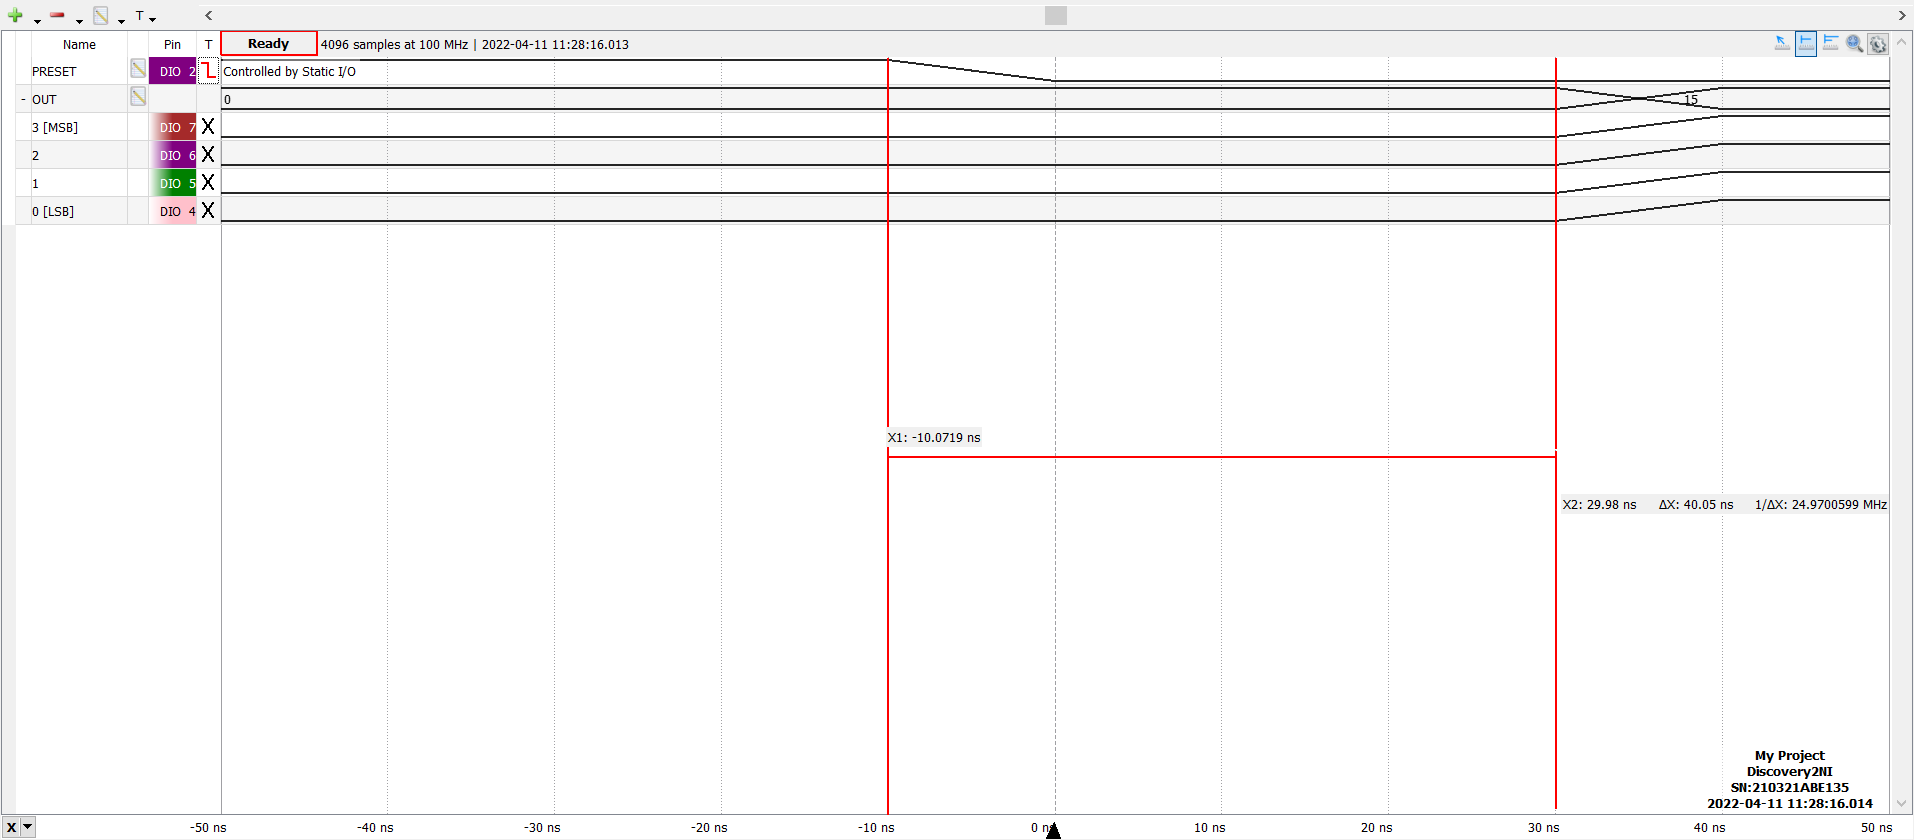
\includegraphics[width=\textwidth]{3.trans}
	\caption{Acquisizione temporale con Logic dei segnali di PRE-BUTTON e i 4 segnali in uscita da un registro a scorrimento di 4 bit come illustrato in \cref{fig: schem_shift}
	\label{fig: Shift_reg_trans}}
\end{figure}
Dalla figura \cref{fig: Shift_reg_trans} vediamo che le commutazioni delle uscite avvengono in maniera sincrona, a un $\Delta T = 40 \si{n\s}$ a partire dalla pressione del pulsante di preset; successivamente le 4 uscite hanno raggiunto lo stato 1111.

\subsection{Verifica del funzionamento tramite clock}\label{sbs: clock_reg}
A questo punto si vuole verificare il funzionamento del registro a scorrimento tramite un segnale di clock.
Possiamo quindi costruire una tabella di verità in funzione del tempo del registro a partire dal periodo $T$ del clock inviato:
\begin{table}[htbp]
\centering
\begin{tabular}{c|cc}
\toprule
$t=t'$ & $t=t' + \Delta T$ & $ $\\
\midrule
\midrule
$Q_0$&$Q_0'$&$Q_0'$\\
$Q_1$&$Q_0$(t=t')&$Q_0$(t=t')\\
$Q_2$&$Q_1$(t=t')&$Q_0$(t=t'-$\Delta T$)\\
$Q_3$&$Q_2$(t=t')&$Q_0$(t=t'-2$\Delta T$)\\
\bottomrule
\end{tabular}
\caption{Tabella "di verità" di un registro a scorrimento, $Q_0'$ è il valore che viene inviato durante l'impulso di clock tramite il D-SWITCH
\label{tab: S-register}}
\end{table}
Come strategia per la verifica, utilizzeremo inizialmente il pulsante di preset per inizializzare tutte le uscite a 1, successivamente imposteremo il D-Switch tramite StaticIO come switch di tipo Push-Pull impostandolo a 0
e invieremo un segnale di clock dell'ordine di 1 Hz. Utilizzeremo quindi Logic per acquisire gli andamenti nel tempo delle uscite.
Dunque ci si aspetta che dopo 3 periodi di clock (3 secondi) a partire da quando l'uscita Q0 diventa 0, tutte le uscite diventino 0, e che aspettando ulteriormente questi valori non cambino.
\begin{figure}[htbp]
\centering
	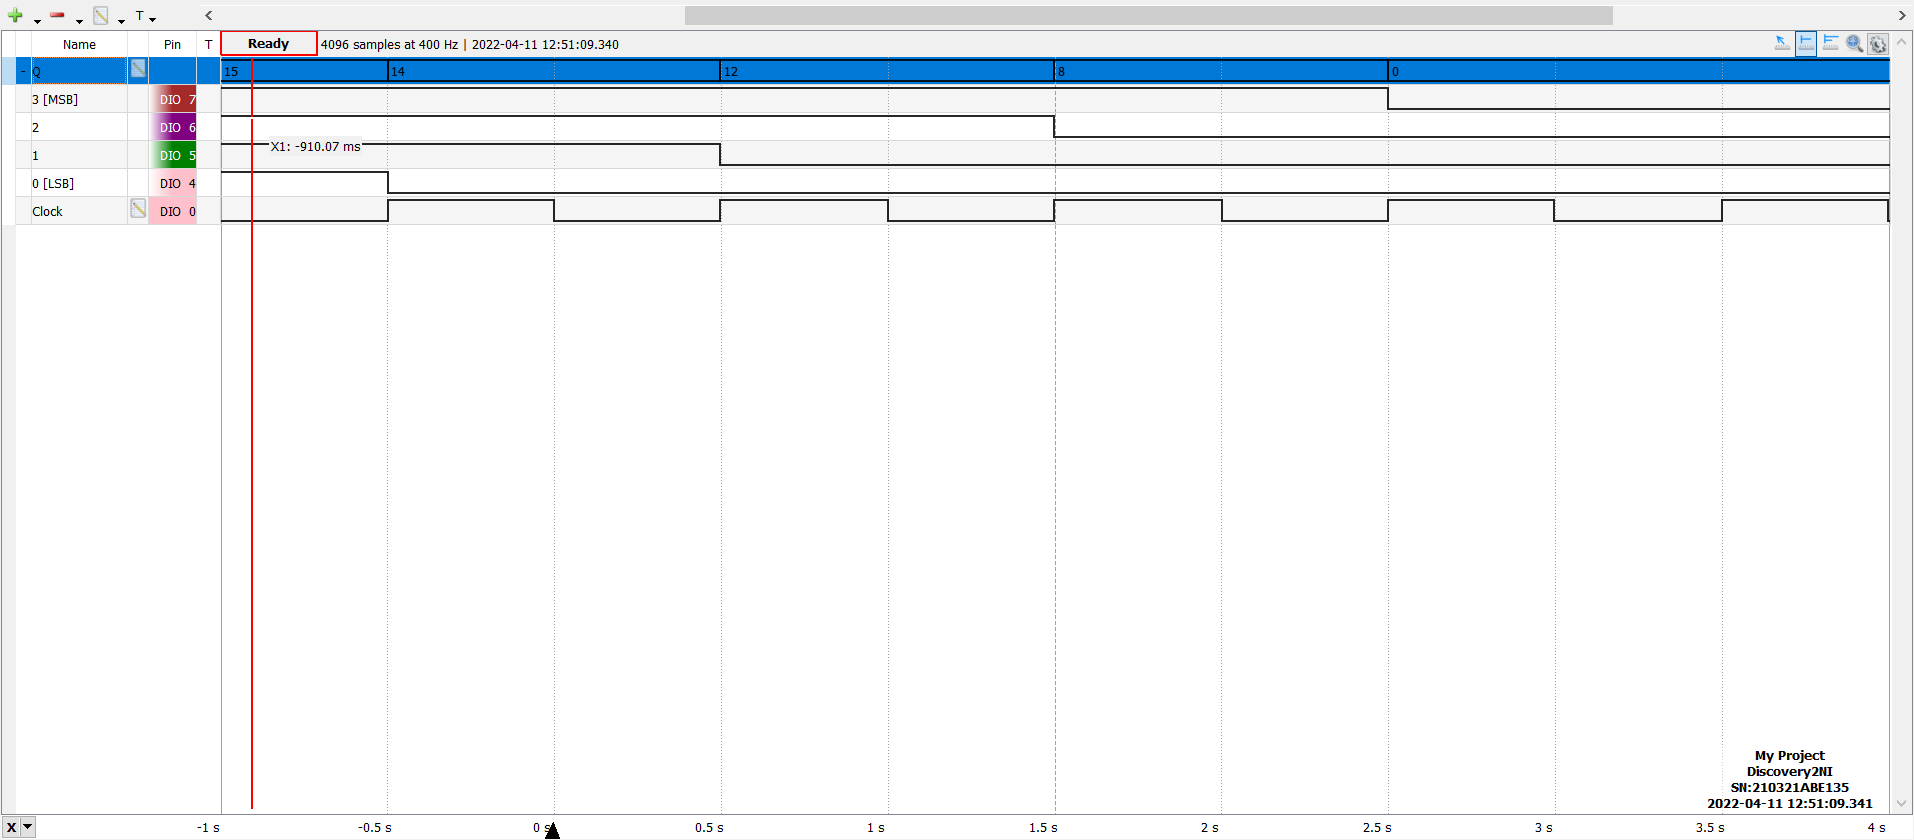
\includegraphics[width=\textwidth]{3.c}
	\caption{Acquisizione temporale con Logic dei segnali in uscita da un registro a scorrimento di 4 bit come spiegato in \cref{sbs: clock_reg} \label{fig: Shift_reg_clock}}
\end{figure}
Dalla \cref{fig: Shift_reg_clock} si verifica quanto detto prima, e le 4 uscite diventano (e si mantengono nel tempo visto che il D-Switch resta fisso a 0) tutte quante 0.
Da questo si intuisce che collegando l'uscita $Q_3$ all'entrata del D-switch, possiamo generare una sequenza periodica.

\subsection{Prevalenza tra gli ingressi D-switch e PRESET}
Utilizzando allo stesso tempo gli ingressi $D$-switch e PRESET del registro
si vede che è l'ultimo a pilotare il segnale in uscita, dal momento che PRESET
è asincrono (indipendente dalla salita del clock). Questo risulta consistente
con la regola generale per cui le architetture asincrone prendono la precedenza
sulle istruzioni sincrone. 

\subsection{Contatore BCD con Flip Flop ad anello}
Dopo aver impostato tutte le uscite a 0, si collega l'uscita $\overline{Q_3}$ all'entrata D del primo Flip-Flop e si  invia un clock di frequenza pari a 1 kHz al circuito.
Ci si aspetta che, prendendo un'uscita a caso, si osservi un segnale di clock di frequenza un quarto di quella di clock: questo effetto è dovuto a come la sequenza viene caricata nel registro a partire dall'uscita $\overline{Q_3}$.
In generale supponendo che nel circuito ci siano in cascata n Flip-Flop, e che tutte le uscite siano inizializzate a 0, in una qualsiasi delle uscite otterrò un clock di frequenza pari a $\frac{f\ped{clk}}{n}$.
\begin{figure}[htbp]
\centering
	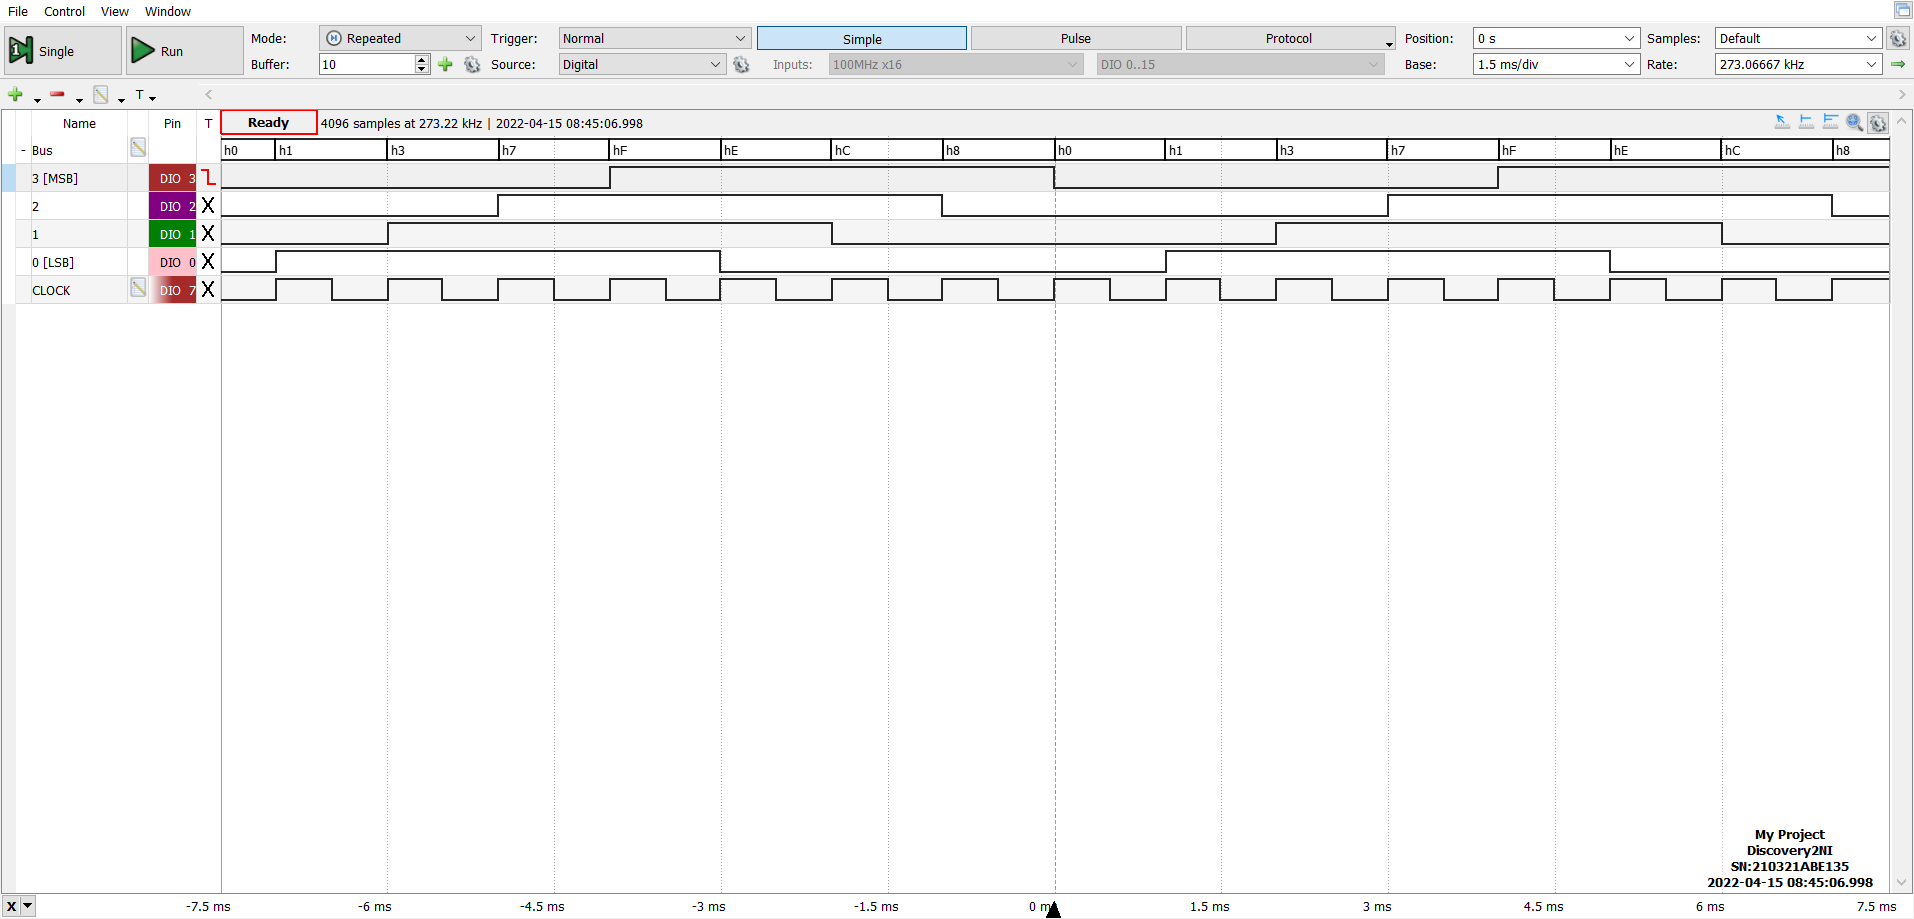
\includegraphics[width=\textwidth]{3.e}
	\caption{Acquisizione temporale con Logic dei segnali in uscita da un registro a scorrimento di 4 bit con l'ultima uscita negata collegata all'entrata del primo flip flop
	\label{fig: Shift_reg_seq}}
\end{figure}

%=======================
\section{Generatore di sequenze pseudo-casuali}
\subsection{Costruzione del circuito}
Si vuole ora costruire un generatore di sequenze pseudo-casuali a 4 bit utilizzando lo shift register costruito in precedenza e una porta XOR; la schematica del circuito che utilizzeremo è riportato in figura \cref{fig: schem_gen}.
\begin{figure}[htbp]
	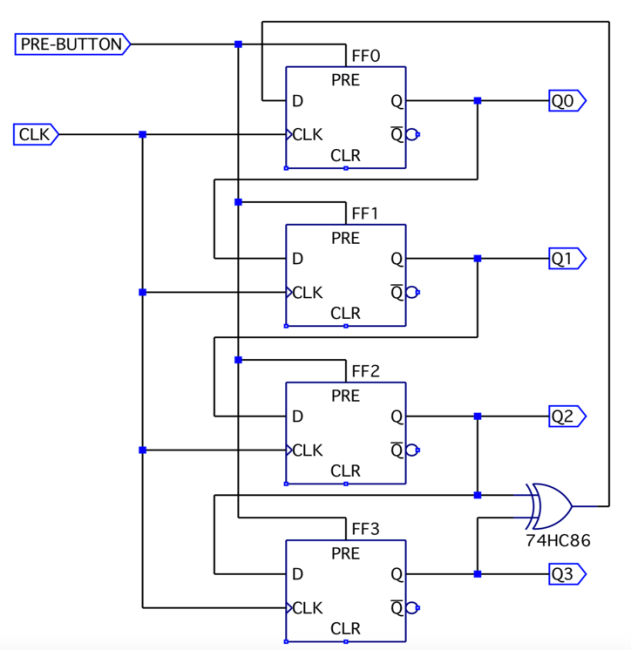
\includegraphics[width=0.6\textwidth]{schem_gen}
	\captionof{figure}{\label{fig: schem_gen}}
\end{figure}

\subsection{Analisi e verifica del funzionamento}
Dopo aver montato il circuito si inizializzano tutti Flip-Flop a 1 e si invia un segnale di clock a 10 kHz per verificare il funzionamento: 
essendo il registro di lunghezza pari a 4 bit, dalla teoria ci aspettiamo che la sequenza si ripeta dopo $2^4 = 16$ eventi al massimo, condizione che si ottiene utilizzando come TAP (segnali in ingresso alla porta XOR, la cui uscita sarà inviata all'entrata D del primo Flip-Flop) le uscite $Q_2$ e $Q_3$. 

\begin{figure}[htbp]
\centering
	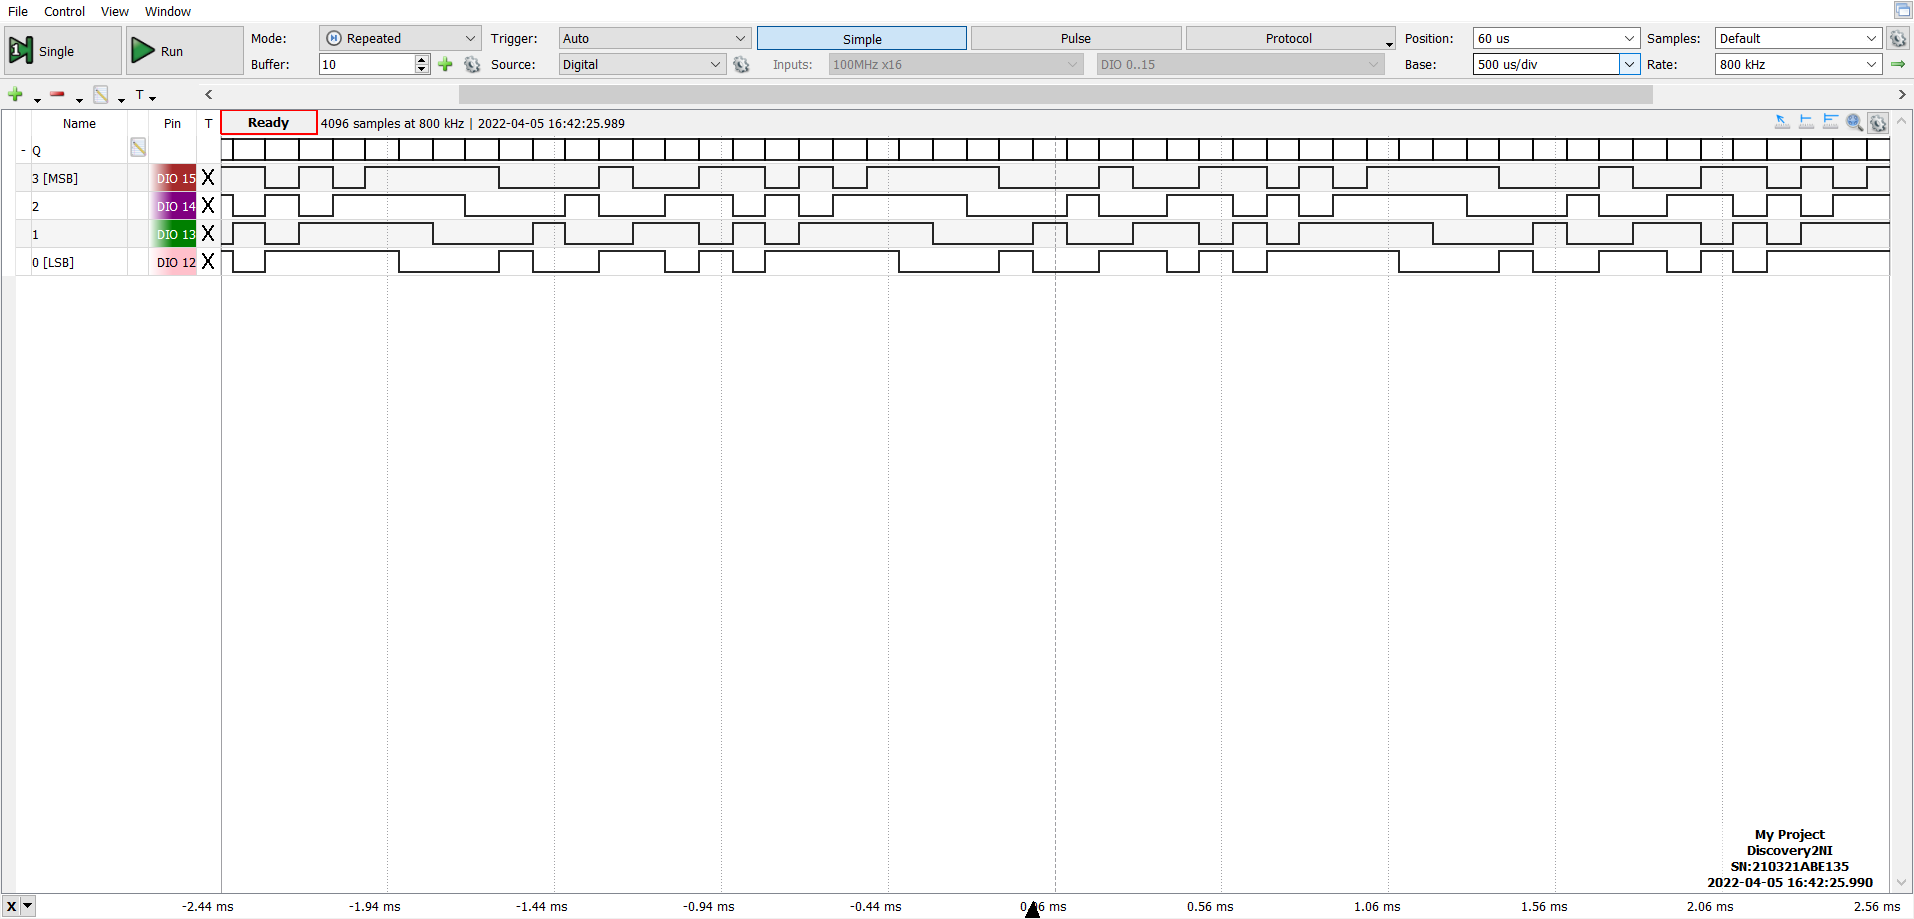
\includegraphics[width=\textwidth]{4.b}
	\caption{\label{fig: TAP_23}Acquisizione temporale con Logic del bus in uscita dal generatore di sequenze psudo-casuale descritto in \cref{fig: schem_gen}}
\end{figure}

Dalla \cref{fig: TAP_23} si verificano le aspettative per cui la sequenza generata a una qualsiasi uscita si ripete ogni 16 periodi di clock (essendo uno shift register la sequenza nelle altre uscite sarà la medesima, solo che saranno sfasate lungo l'asse temporale le une con le altre).
\subsection{Studio delle sequenze generabili con diverse condizioni iniziali}
Si provano quindi altre combinazioni di TAP, per verificare che la scelta di utilizzare l'uscita $Q_2$ e $Q_3$ produce una sequenza più lunga rispetto a qualunque altra configurazione
\begin{figure}[htbp]
\centering
	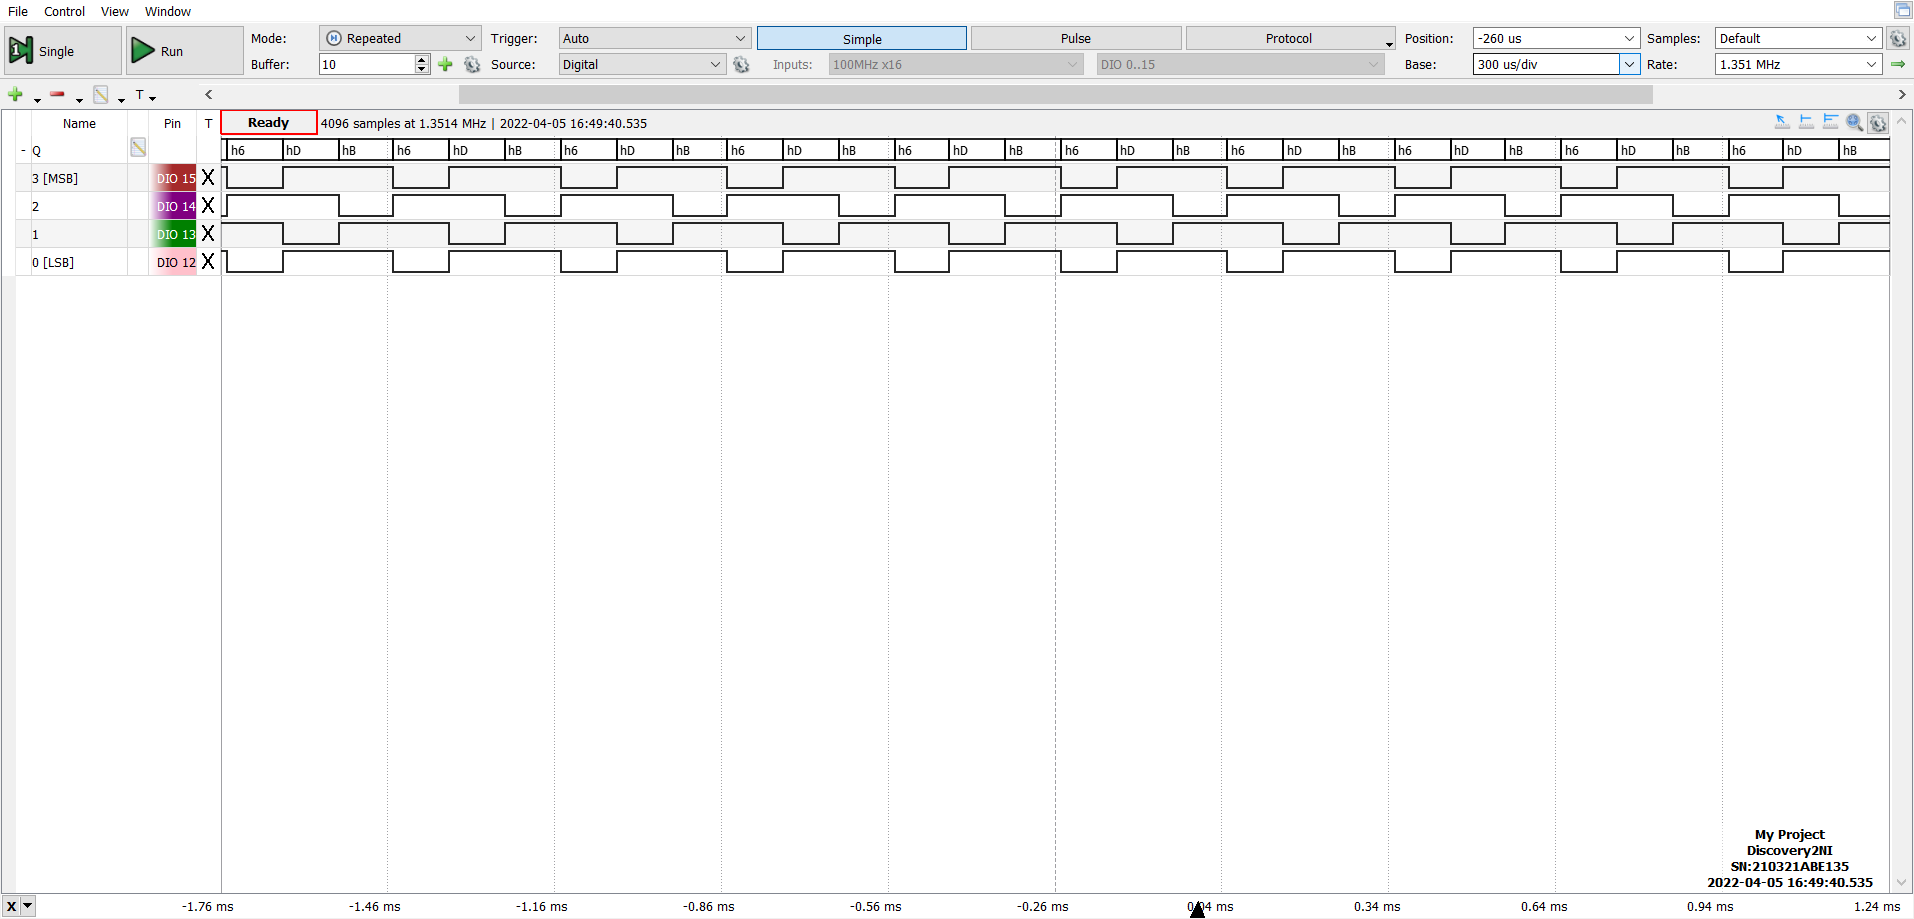
\includegraphics[width=\textwidth]{4.b_10}
	\caption{Acquisizione temporale con Logic del bus in uscita dal generatore di sequenze psudo-casuale con TAP sulle uscite $Q_0$ e $Q_1$, la sequenza si ripete ogni 4 eventi
	\label{fig: TAP_10}}
\end{figure}
\begin{figure}[htbp]
	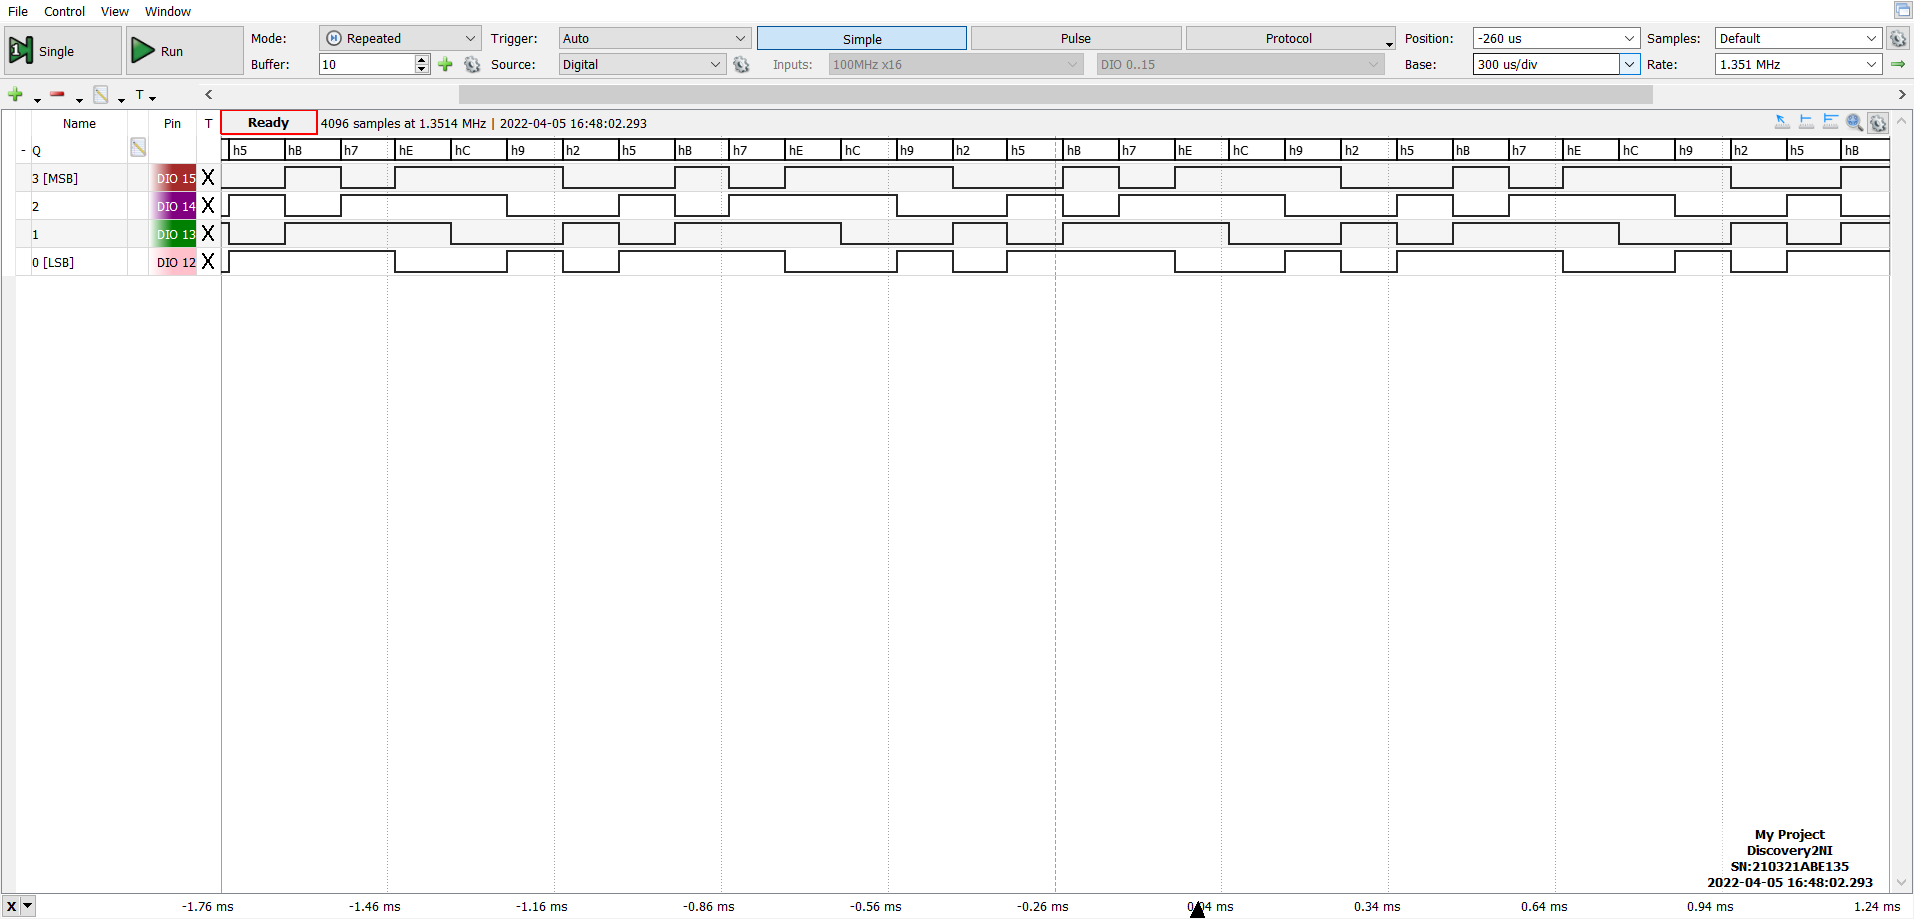
\includegraphics[width=\textwidth]{4.b_21}
	\caption{Acquisizione temporale con Logic del bus in uscita dal generatore di sequenze psudo-casuale con TAP sulle uscite $Q_2$ e $Q_1$, la sequenza si ripete ogni 8 eventi
	\label{fig: TAP_21}}
\end{figure}
\begin{figure}[htbp]
\centering
	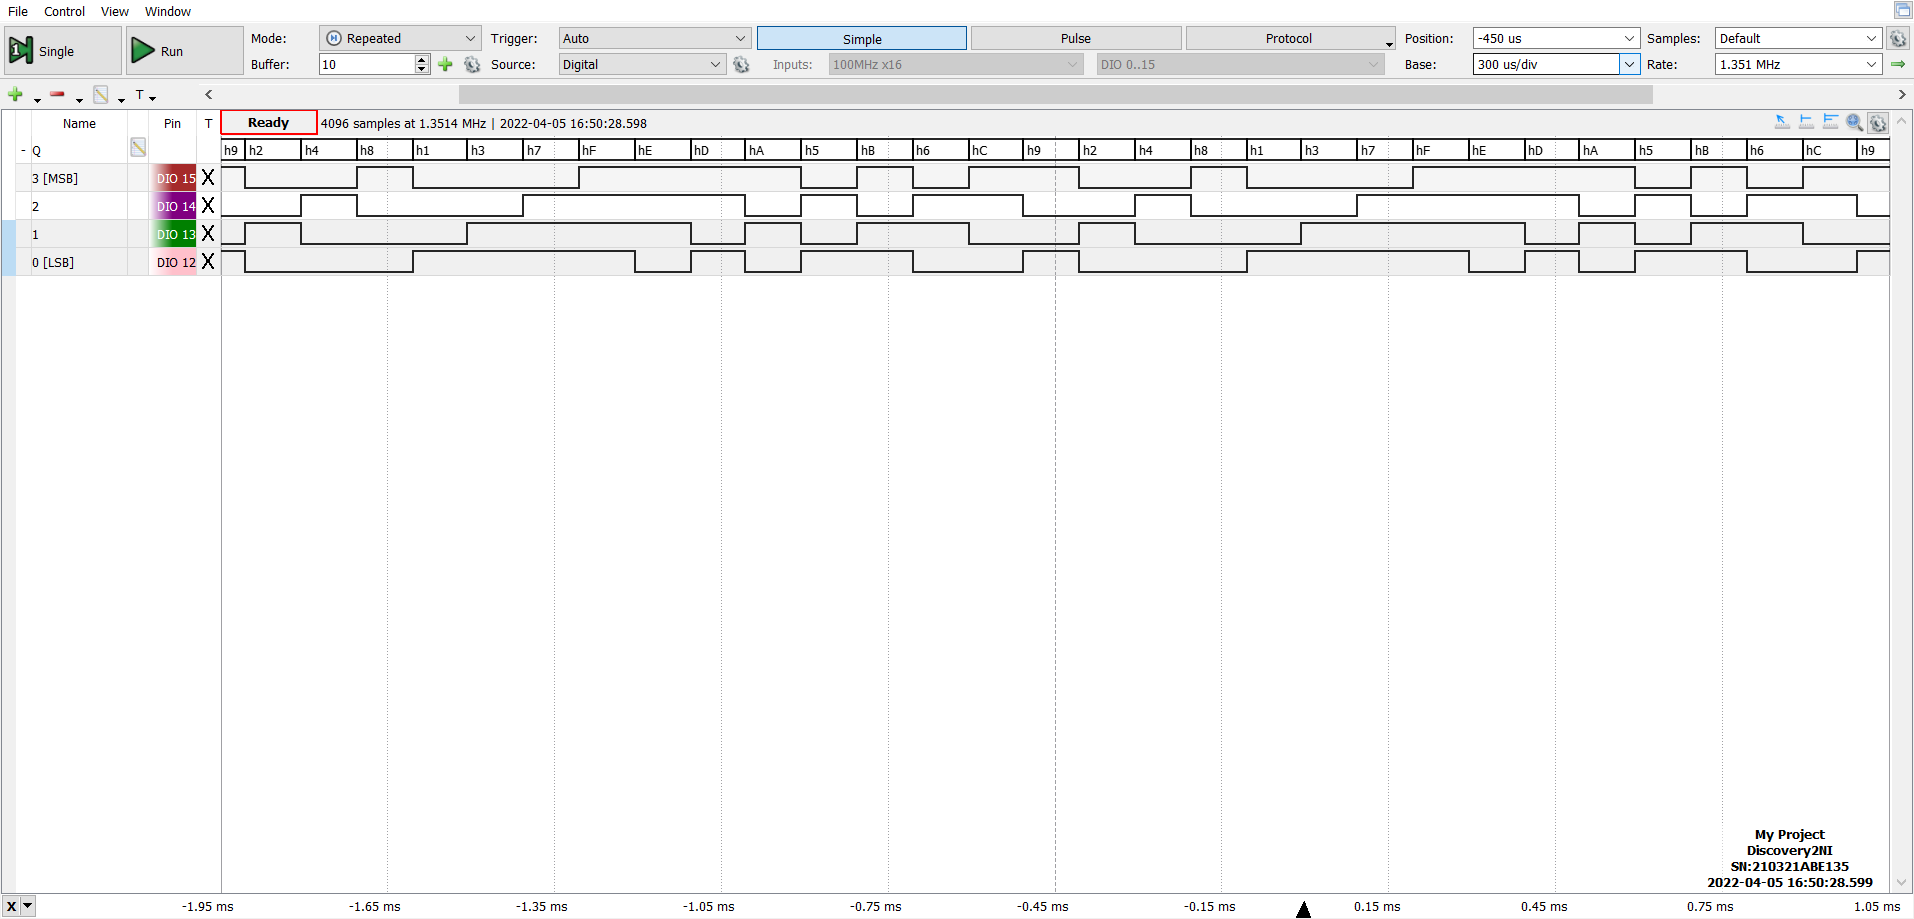
\includegraphics[width=\textwidth]{4.b_30}
	\caption{Acquisizione temporale con Logic del bus in uscita dal generatore di sequenze psudo-casuale con TAP sulle uscite $Q_0$ e $Q_3$, la sequenza si ripete ogni 16 eventi \label{fig: TAP_30}}
\end{figure}

%=======================
\section{Divisori di frequenza con contatori binari}
\subsection{Costruzione del circuito}
Si intende costruire un divisore di frequenza a partire da un contatore binario a 4 bit, utilizzando l'integrato SN74LS163, presente in \cref{fig: schem_counter}. Si vuole innanzitutto verificarne il funzionamento. 
\begin{figure}[htbp]
\centering
	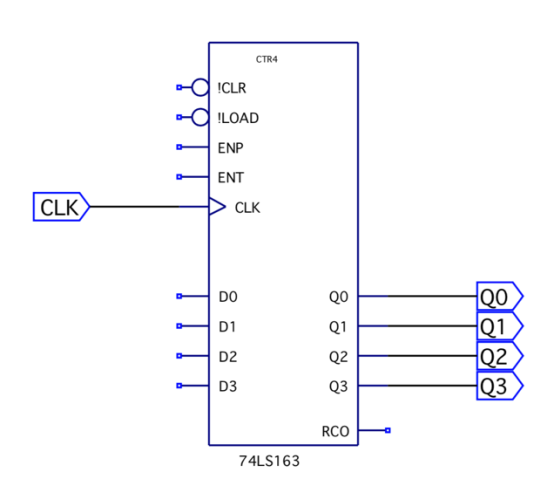
\includegraphics[width=\textwidth]{schem_con}
	\caption{\label{fig: schem_counter}}
\end{figure}

\subsection{Verifica del ciclo di funzionamento dei contatori}
Dopo aver montato il circuito utilizziamo la funzione Pattern di Waveform per inviare un segnale di clock di frequenza pari a 10 kHz al pin di clock (CLK) del contatore, e utilizzeremo Logic per acquisire le uscite $Q_0$->$Q_3$.
Essendo un contatore a 4 bit, ci si aspetta che il Bus conti dallo stato 0000 (0 in decimale) fino allo stato 1111 (15 in decimale).
Per questo motivo utilizzeremo un formato di Bus esadecimale per verificare che il circuito generi tutti gli stati possibili (0->F).
\begin{figure}[htbp]
\centering
	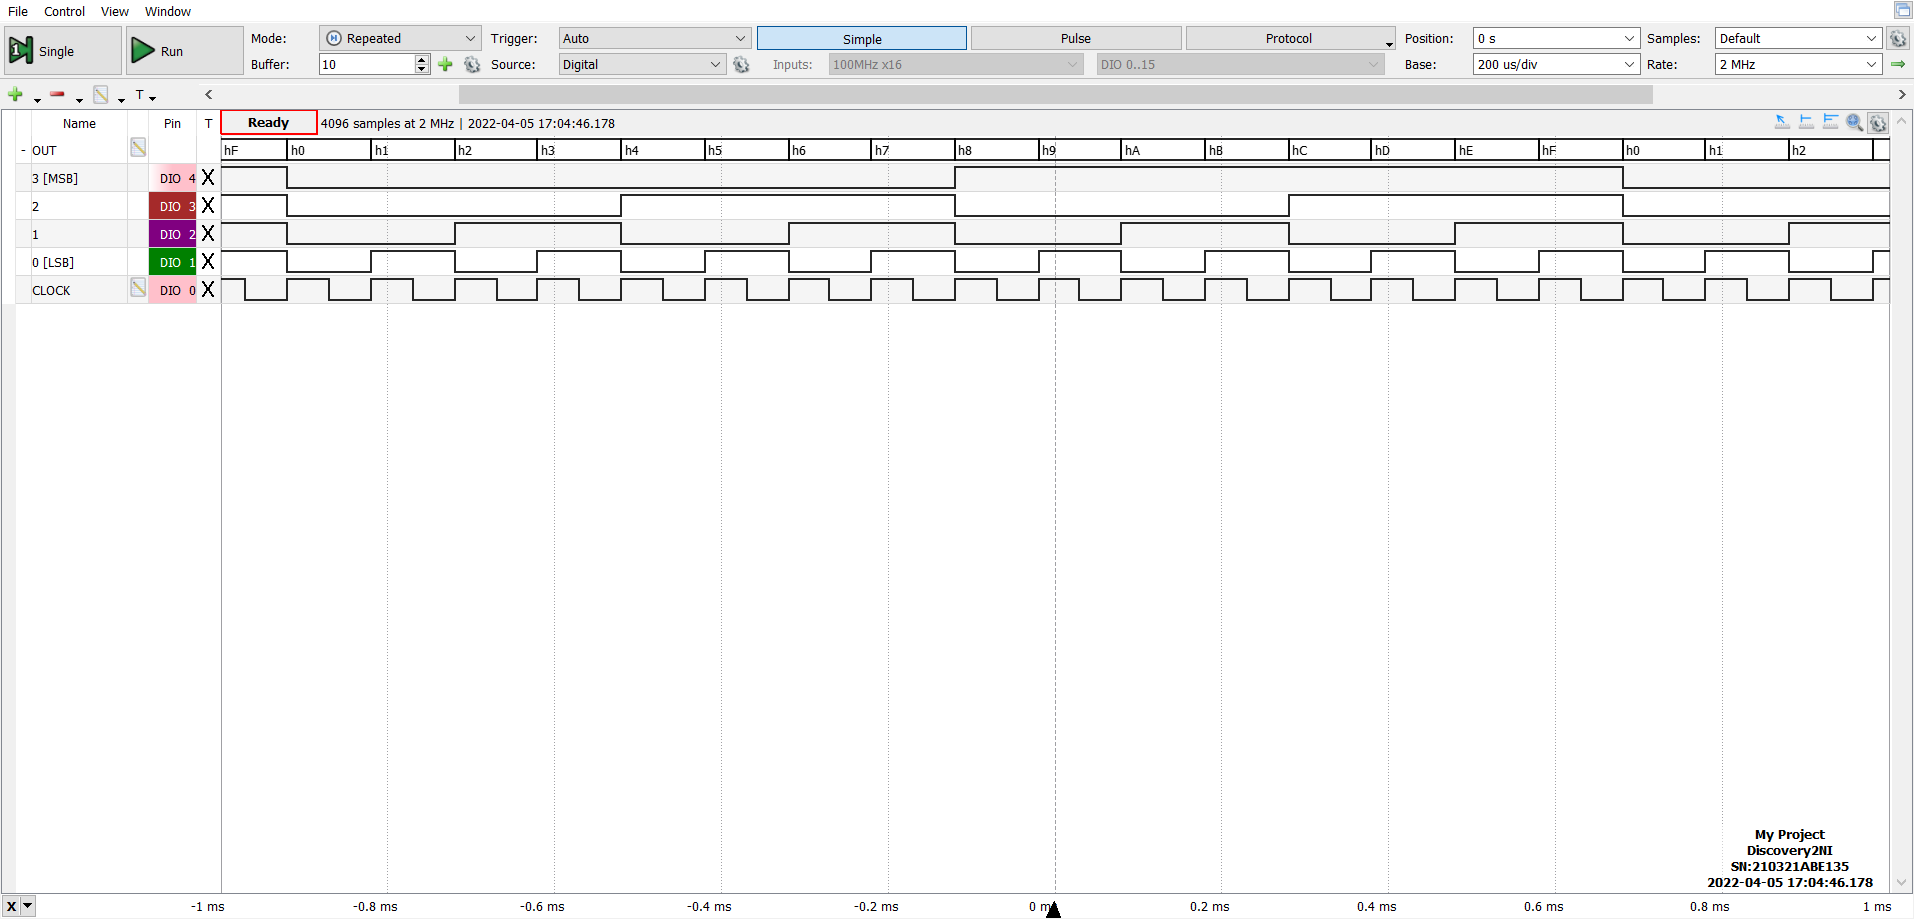
\includegraphics[width=\textwidth]{5.b}
	\caption{Acquisizione temporale con Logic del bus in uscita dal contatore, con frequenza di clock pari a 10 kHz \label{fig: Count_Clock}}
\end{figure}
Dalla \cref{fig: Count_Clock} si può notare che il comportamento del circuito è come atteso, e che gli stati del bus in uscita comprendono tutti i valori in ordine crescente della numerazione esadecimale 
\subsection{Verifica della divisione in frequenza}

Dato che il contatore incrementa di 1 ad ogni evento di clock, il bit di ordine n avrà come frequenza la metà di quella del bit di ordine n-1.
Avendo noi un BUS composto da 4 bit, ci si aspetta che le frequenze ottenute siano $\frac{f_clock}{2}$ (per il LSB),$\frac{f_clock}{4}$,$\frac{f_clock}{8}$ e $\frac{f_clock}{16}$ (per il MSB).
Sempre facendo riferimento all  \cref{fig: Count_Clock} si può notare come le uscite del contatore si comportino da divisori in frequenza: infatti i periodi che si trovano analizzando l'acquisizione sono 2 (LSB), 4, 8 e 16 (MSB) volte il periodo del clock.
\subsection{Transizione sincrona del contatore}
Utilizziamo quindi la funzione di trigger di Logic e la impostiamo in modo tale che l'acquisizione cominci quando il segnale presente in $Q_3$ cambia da 1 a 0 in modo da poter studiare gli eventuali ritardi delle singole uscite nella transizione F->0 e verificare il comportamento sincrono del contatore.
\begin{figure}[htbp]
\centering
	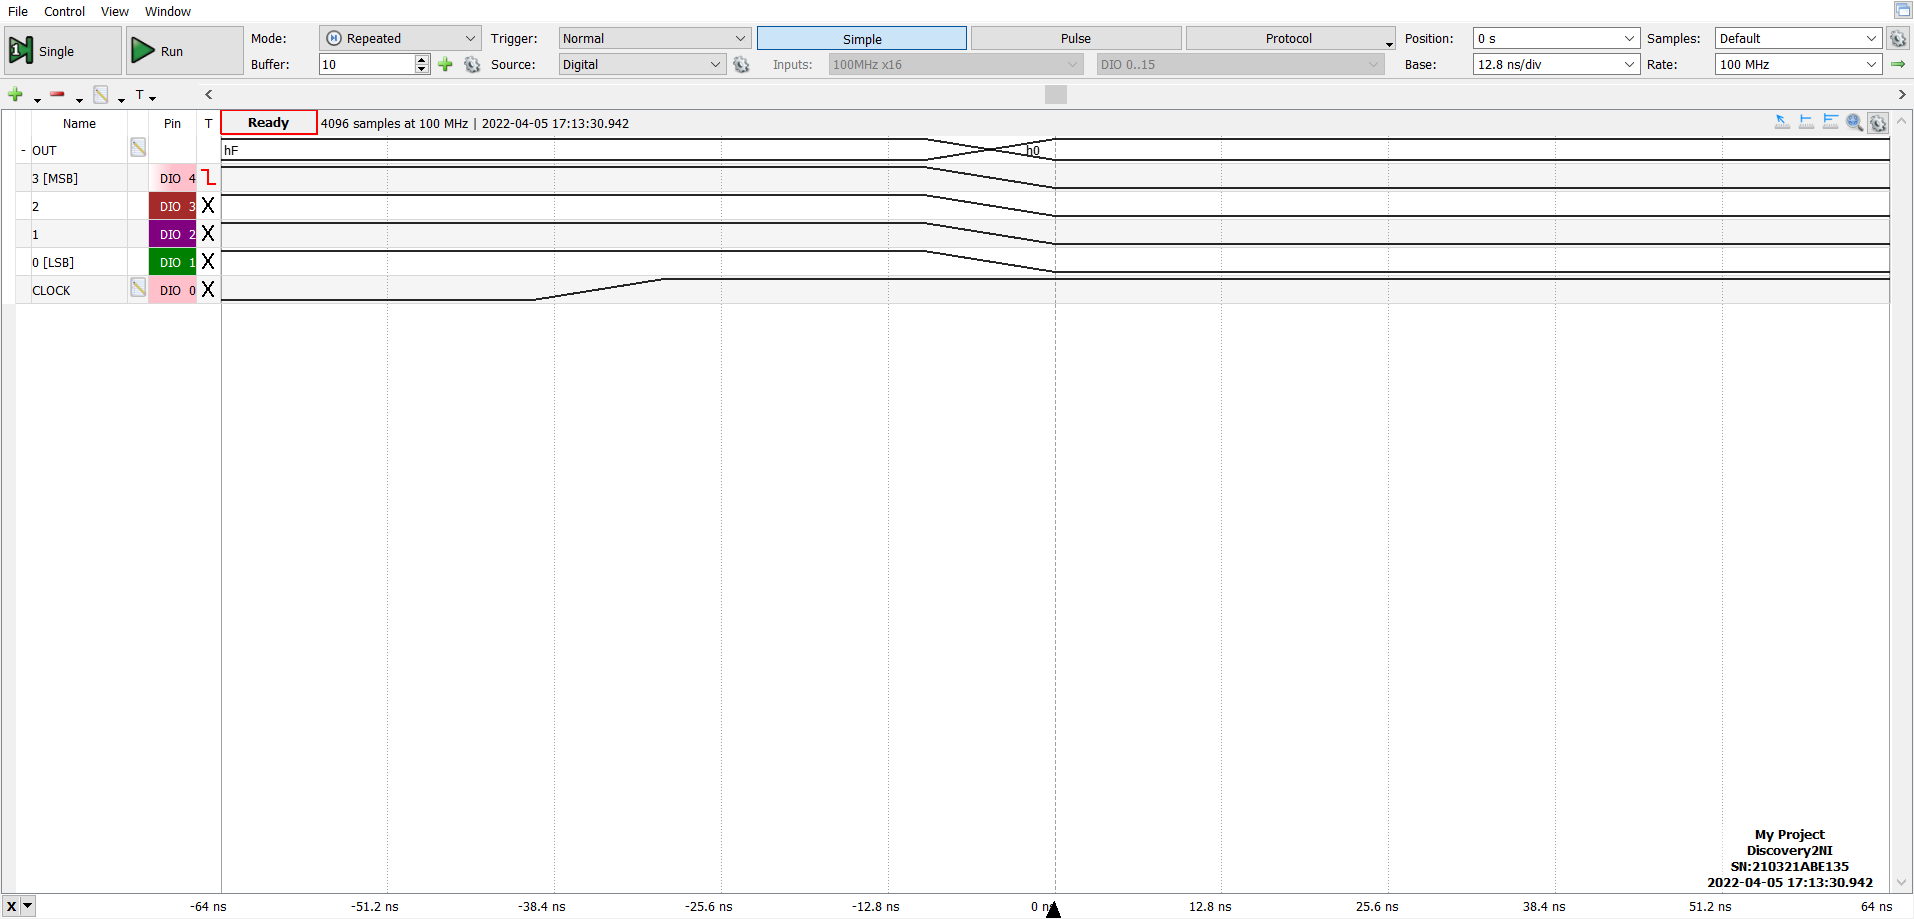
\includegraphics[width=\textwidth]{5.d}
	\caption{Acquisizione temporale con Logic del bus in uscita dal contatore durante la transizione 15->0; dall'immagine possiamo notare il comportamento sincrono della commutazione delle uscite del contatore \label{fig: Count_150}}
\end{figure}
Dalla \cref{fig: Count_150} possiamo infatti vedere che la transizione è sincrona e il passaggio di stato 1->0 avviene contemporaneamente in ogni uscita.
\subsection{Costruzione di un divisore di frequenza 1/10}
Si vuole quindi realizzare un divisore in frequenza, che generi un segnale di periodo pari a 10 volte quello di clock: per farlo utilizzeremo il pin CLEAR del contatore, il quale quando viene inviato un segnale Low resetta il contatore allo stato 0000.
\begin{figure}[htbp]
\centering
	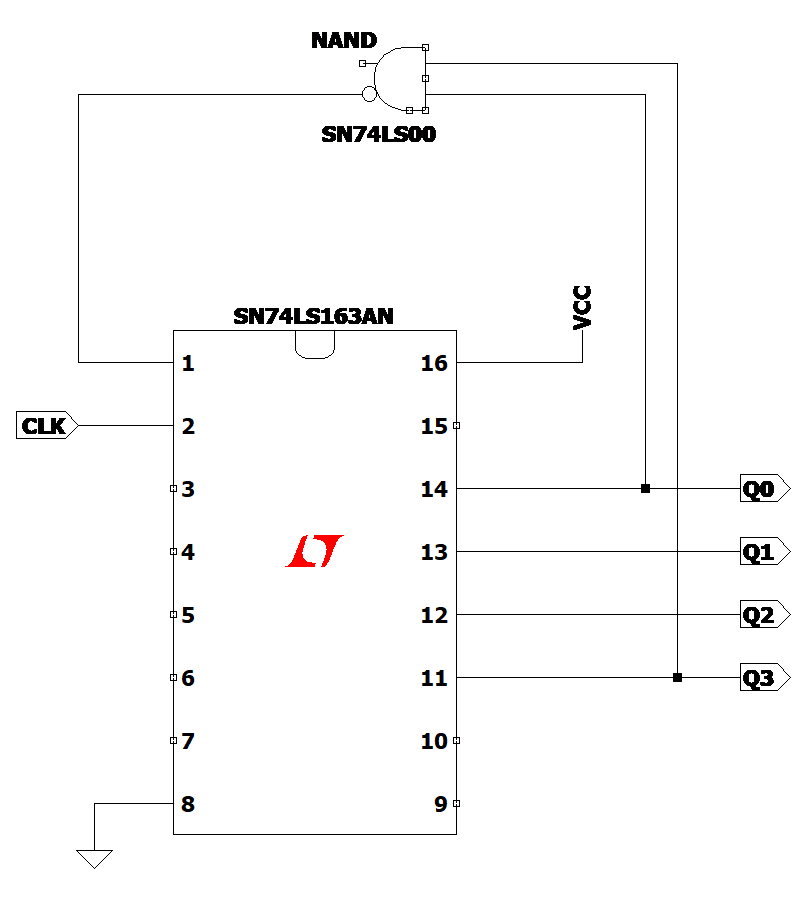
\includegraphics[width=\textwidth]{Draft1}
	\label{schem: 10_div}
	\caption{Schematica utilizzata per il divisore per 10 di frequenza}
\end{figure}
È quindi necessario che il contatore conti un totale di 10 stati e poi si resetti, per cui partendo dallo 0, dobbiamo imporre la condizione che arrivati allo stato 9, il contatore riceva l'impulso di Clear (che ricordiamo essere Active Low).
Per farlo utilizzeremo una porta NAND (utilizzando l'integrato SN74LS00) ai cui 2 ingressi invieremo il LSB e il MSB e invieremo l'uscita al pin di Clear. In questo modo, quando il contatore arriva a 9 (1001) il pin di Clear riceverà un segnale Low e il circuito si azzererà; pertanto la frequenza del segnale Clear sarà un decimo di quella di clock
Inoltre essendo il segnale di Clear sullo stato Low solamente quando il bus in uscita registra lo stato 1001, mi aspetterò un Duty Cycle pari al $90 \percent$
Si costruisce quindi il circuito presente in \cref{schem: 10_div}.
\begin{figure}[htbp]
\centering
	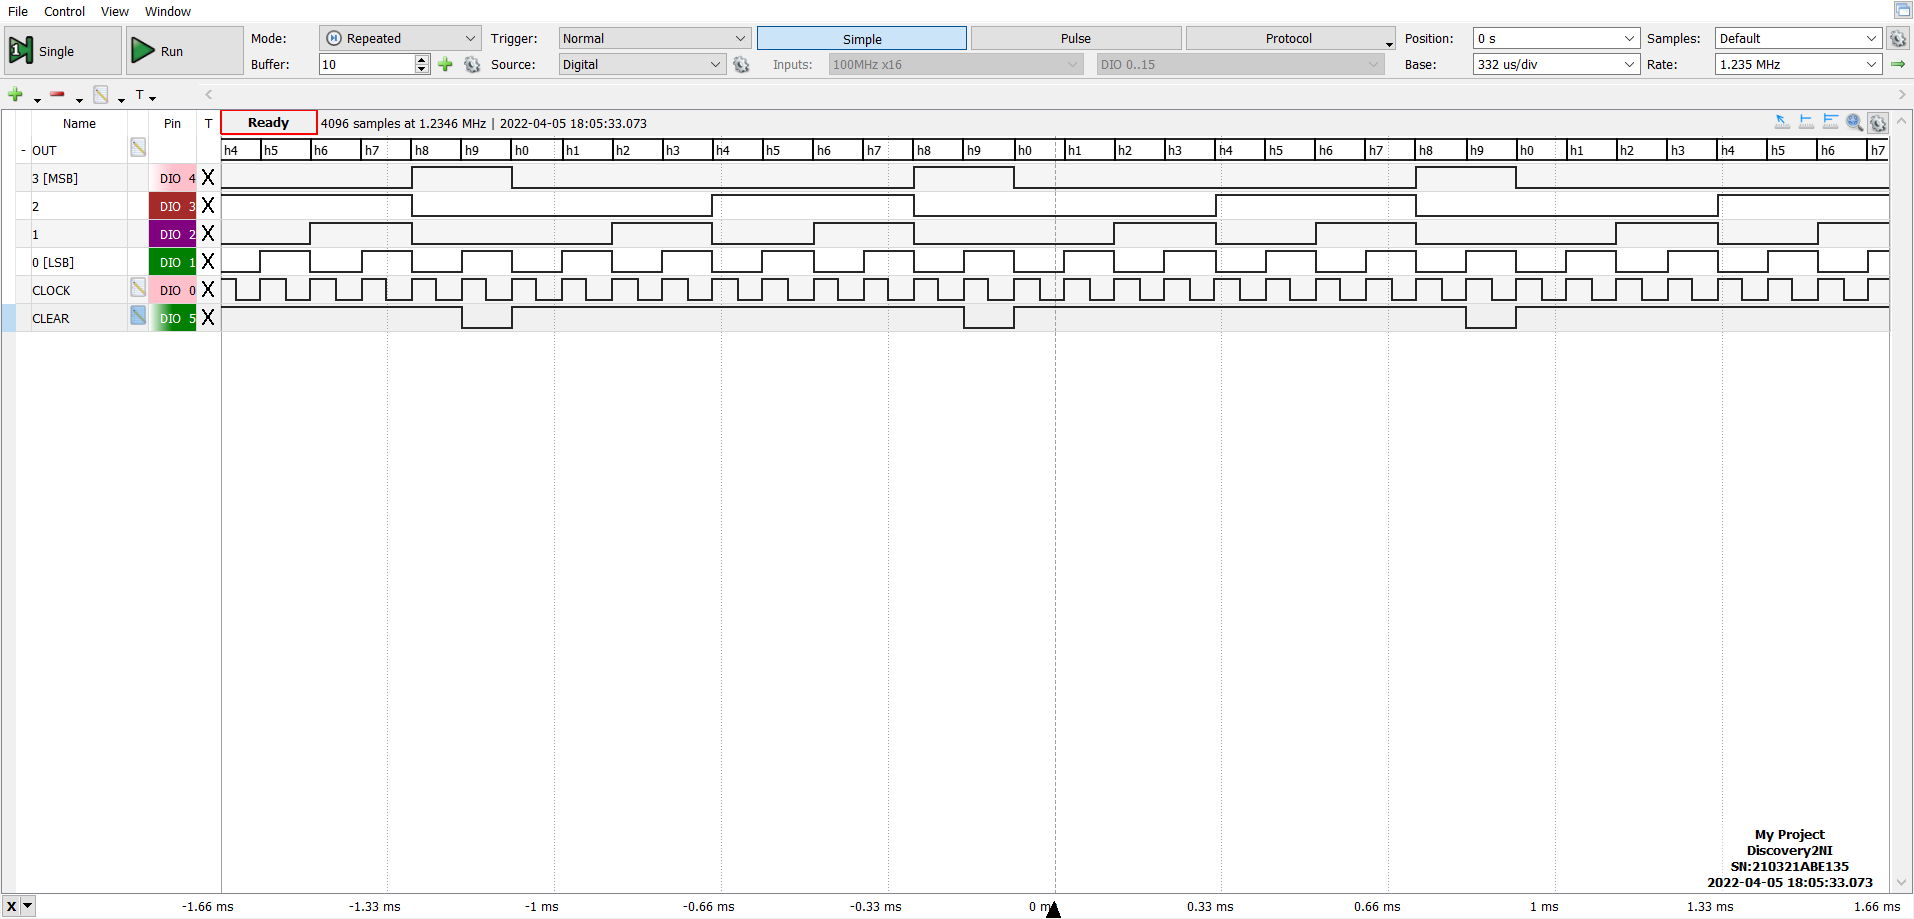
\includegraphics[width=\textwidth]{5.e}
	\caption{Acquisizione temporale con Logic del bus in uscita dal circuito che conta fino a 10; si può notare che il segnale in entrata nel pin Clear ha effettivamente periodo pari a 10 volte quello del clock \label{fig: Count_10th}}
\end{figure}
Come prima, si utilizza la funzione Logic per acquisire il Bus dei 4 bit in uscita, il clock e il bit di Clear.
Osservando l'acquisizione presente in \cref{fig: Count_10th}, possiamo concludere come da aspettative che il segnale presente su clear ha una frequenza pari a $\frac{f_{clock}}{10}$ e Duty Cycle pari al $90 \percent$.
\subsection{Divisore di frequenza programmabile con RCO}
\begin{figure}[htbp]
\centering
	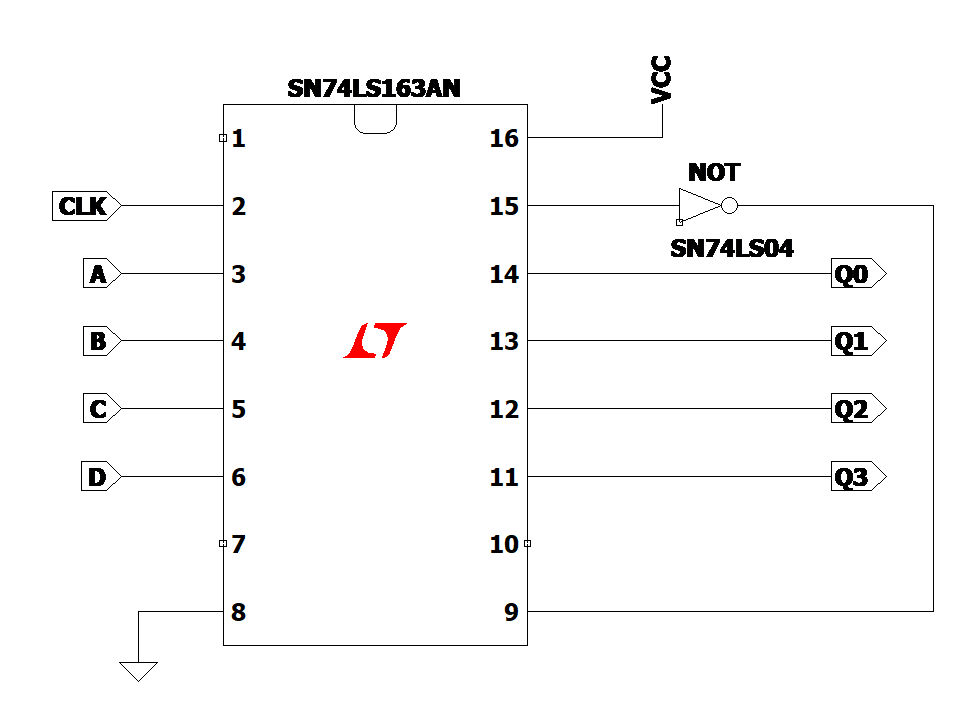
\includegraphics[width=\textwidth]{Draft2}
	\caption{Schematica utilizzata per il divisore di frequenza programmabile}
\end{figure}

\subsection{Misura dei tempi caratteristici del divisore RCO}
\subsection{Analisi e verifica del comportamento del divisore RCO}

%=======================
\section{Sintetizzatore musicale}

%=======================
\section*{Conclusioni e commenti finali}
Si è riusciti a verificare il corretto funzionamento di circuiti logici
sequenziali di crescente complessità e svariate applicazioni (e.g.
crittografia, sistemi di controllo e misura) costruiti con porte NAND, XOR,
D-Latch e contatori sincroni.
In particolare sono stati realizzati e studiati un D-Latch, uno shift-register
con positive edge-triggered D-FF, un generatore di sequenze pseudocasuali e
alcuni tipi di divisore di frequenza con contatori binari.
Inoltre si è riusciti ad apprezzare l'effetto dei tempi di propagazione
delle porte sul loro comportamento, seppur in maniera limitata dalla bassa
risoluzione temporale dell'AD2.

%=======================
\section*{Dichiarazione}
I firmatari di questa relazione dichiarano che il contenuto della relazione \`e
originale, con misure effettuate dai membri del gruppo, e che tutti i firmatari
hanno contribuito alla elaborazione della relazione stessa.

\end{document}
